\documentclass{article}
% translate with >> pdflatex -shell-escape <file>

% This file is an extract of the PGFPLOTS manual, copyright by Christian Feuersaenger.
% 
% Feel free to use it as long as you cite the pgfplots manual properly.
%
% See
%   http://pgfplots.sourceforge.net/pgfplots.pdf
% for the complete manual.
%
% Any required input files (for <plot table> or <plot file> or the table package) can be downloaded
% at
% http://www.ctan.org/tex-archive/graphics/pgf/contrib/pgfplots/doc/latex/
% and
% http://www.ctan.org/tex-archive/graphics/pgf/contrib/pgfplots/doc/latex/plotdata/

\usepackage{pgfplots}
\pgfplotsset{compat=newest}

\pagestyle{empty}

\begin{document}
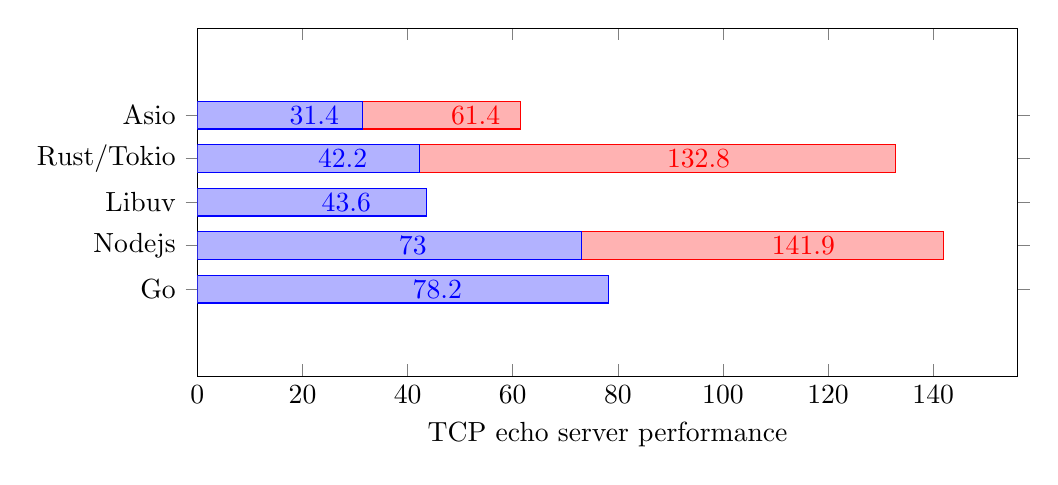
\begin{tikzpicture}
  \begin{axis}[
    y dir=reverse,
    xbar stacked,
    xbar, xmin=0,
    %hide x axis,
    bar shift=0pt,
    width=12cm, height=6cm, enlarge y limits=0.5,
    xlabel={TCP echo server performance},
    symbolic y coords={Asio,Rust/Tokio,Libuv,Nodejs,Go},
    ytick=data,
    %bar width=1cm,
    nodes near coords,
    nodes near coords align={horizontal},
    ]
    \addplot coordinates {
       (31.4,Asio)
       (42.2,Rust/Tokio)
       (43.6,Libuv)
       (73.0,Nodejs)
       (78.2,Go)
    };
    \addplot coordinates {
       (30.0,Asio)
       (90.6,Rust/Tokio)
       (0.0,Libuv)
       (68.9,Nodejs)
       (0.0,Go)
    };
  \end{axis}
\end{tikzpicture}
\end{document}
